\documentclass[a4paper,12pt]{article}

%\addtolength{\voffset}{-4cm}
%\usepackage[spanish]{babel}
\usepackage{amsmath}
\usepackage{mycmds}
\usepackage{graphicx}
\pagestyle{headings}

\author{Jos\'e Angel de Bustos P\'erez}

\frenchspacing

\hyphenation{si-guien-te apro-xi-ma-cio-nes FORTRAN double intGrado 
dblDerivada dblResultado intNMI intOrden dblMatriz Newton intResultado
cabezera coor-de-na-das de-pen-dien-do di-men-sio-na-do re-pre-sen-tan-do}

\begin{document}

\thispagestyle{empty}

\begin{center}
\Huge{Cryptography I - Coursera} \\[.75cm]
\large{Week 1 - Problem Set}
\end{center}

\large 
\begin{flushright}
\yo \\
$<$jadebustos@gmail.com$>$\\ \ \\ 
Versi\'on $1.0$, \today .\\
\textbf{\LaTeXe}
\end{flushright}

\normalsize

\textbf{Question 1} \\

Data compression is often used in data storage and transmission. Suppose you want to use data compression in conjunction with encryption. Does it make more sense to:
%
\begin{itemize}
\item Encrypt then compress.
\item \textbf{Compress then encrypt}.
\item The order does not matter -- either one is fine.
\item The order does not matter -- neither one will compress the data.
\end{itemize}

\textbf{Solution}\\

Compress before encrypting has the following advantages:
%
\begin{enumerate}
\item Compress used to reduce patterns so the plain text will offer less redundancies that could not being spread to cipher text if encrypt algoright would not be semantically secure.
\item The amount of data will be smaller so the encryption will be more efficient.
\end{enumerate}
%
After encryption cyphertexts used to look like random strings and therefore the only oportunity for compression is prior to encryption.\\

\ \newpage

\textbf{Question 2} \\

Let $G:\{0,1\}^{s}\rightarrow \{0,1\}^{n}$ be a secure PRG. Which of the following is a secure PRG (there is more than one correct answer):
%
\begin{enumerate}
\item $G'(k)=G(k\oplus 1^{s})$
\item $G'(k)=G(k\oplus 1^{n})$
\item $G'(k)=G(0)$
\item $G'(k)=G(k)[0,…,n - 2]$     (i.e., $G′(k)$ drops the last bit of $G(k)$)
\item $G'(k)=G(k)\mid \mid G(k)$     (here $\mid \mid$ denotes concatenation)
\item $G'(k)=G(k)\mid \mid 0$     (here $\mid \mid$ denotes concatenation)
\item $G'(k_{1},k_{2})=G(k_{1})\mid \mid G(k_{2})$     (here $\mid \mid$ denotes concatenation)
\item $G'(k,k)=$ reverse $G(k)$ where reverse $x$ reverses the string $x$ so that the first bit of $x$ is the last bit of reverse$(x)$, the second bit of $x$ is the second to last bit of reverse$(x)$, and so on.
\end{enumerate}

\textbf{Solution} \\

The secure PRGs are:
%
\begin{enumerate}
\item $G'(k)=G(k\oplus 1^{s})$. A distinguisher for $G'$ gives a distinguisher for $G$.
\item $G'(k)=G(k\oplus 1^{n})$. A distinguisher for $G'$ gives a distinguisher for $G$.
\item $G'(k_{1},k_{2})=G(k_{1})\mid \mid G(k_{2})$ (here $\mid \mid$ denotes concatenation). A distinguisher for $G'$ gives a distinguisher for $G$.
\item $G'(k)=G(k)[0,…,n - 2]$ (i.e., $G'(k)$ drops the last bit of $G(k)$). A distinguisher for $G'$ gives a distinguisher for $G$.
\item $G'(k,k)=$ reverse $G(k)$ where reverse $x$ reverses the string $x$ so that the first bit of $x$ is the last bit of reverse$(x)$, the second bit of $x$ is the second to last bit of reverse$(x)$, and so on. A distinguisher for $G'$ gives a distinguisher for $G$.
\end{enumerate}
%
\ \newpage
%
The insecure PRGs are:
%
\begin{enumerate}
\item $G'(k)=G(0)$. A distinguisher will output \emph{not ramdon} whenever its input is equal to $G(0)$.
\item $G'(k)=G(k)\mid \mid G(k)$ (here $\mid \mid$ denotes concatenation). A distinguisher will output \emph{not ramdon} whenever the first $n$ bits are equal to the last $n$ bits.
\item $G'(k)=G(k)\mid \mid 0$ (here $\mid \mid$ denotes concatenation). A distinguisher will output \emph{not ramdon} whenever its input is $0$.
\end{enumerate}

\textbf{Question 3} \\

Let $G:K\rightarrow \{0,1\}^{n}$ be a secure PRG. Define $G'(k_{1},k_{2})=G(k_{1})\wedge G(k_{2})$ where $\wedge$ is the bit-wise AND function. Consider the following statistical test $A$ on $\{0,1\}^{n}$:
%
\begin{quote}
$A(x)$ outputs $LSB(x)$, the least significant bit of x.   
\end{quote}
%
What is $Adv_{PRG}[A,G']$? You may assume that $LSB(G(k))$ is 0 for exactly half the seeds $k$ in $K$.\\ 

Note: Please enter the advantage as a decimal between 0 and 1 with a leading 0. If the advantage is $\frac{3}{4}$, you should enter it as 0.75.\\

\textbf{Solution} \\

\begin{center}
%
\begin{tabular}{c|c|c}
X & Y & AND \\
\hline
 $0$ & $0$ & $0$ \\
 $0$ & $1$ & $0$\\
 $1$ & $0$ & $0$\\
 $1$ & $1$ & $1$ 
\end{tabular}
%
\end{center}

\begin{equation*}
Adv_{PRG}[A,G'] = |Pr[\overbrace{A(G'(k_{1},k_{2}))=1}^{k_{1},k_{2} \xleftarrow{r} K}] - Pr[\overbrace{A(r)=1}^{r \leftarrow \{0,1\}^{n}}]|
\end{equation*}
%
So:
%
\begin{eqnarray*}
Pr[A(G'(k_{1},k_{2}))=1] & = & Pr[(A(G(k_{1})\wedge G(k_{2})))=1] = Pr[(LSB(G(k_{1})\wedge G(k_{2})))=1] = \\
 & = & Pr[(LSB(G(k_{1}))\wedge LSB(G(k_{2})))=1]
\end{eqnarray*}
%
Due to we assume that $LSB(G(k)) = 0$ for exactly half of the seeds $k \in K$ then:
%
\begin{eqnarray}
Pr[LSB(G(k))=0] & = & \frac{1}{2} \label{eqn:prob-zero} \\
Pr[LSB(G(k))=1] & = & \frac{1}{2}  \label{eqn:prob-one}
\end{eqnarray}
%
There are $4$ possible values that the AND function can take. Only one of them is $1$, and how $0$ and $1$ have the same probability (equation ($\ref{eqn:prob-zero}$) and ($\ref{eqn:prob-one}$)):
%
\begin{equation*}
Pr[(LSB(G(k_{1}))\wedge LSB(G(k_{2})))=1] = \frac{1}{4}  
\end{equation*}
%
So:
%
\begin{equation*}
Pr[A(r)=1] = Pr[LSB(r)=1] = \frac{1}{2}  
\end{equation*}
%
Due to $r\leftarrow \{0,1\}^{n}$.

\begin{equation*}
Adv_{PRG}[A,G'] = |Pr[A(G'(k_{1},k_{2}))=1] - Pr[A(r)=1]| = |\frac{1}{4}-\frac{1}{2}| = \frac{1}{4}
\end{equation*}

\ \\
\textbf{Question 4} \\

Let $(E,D)$ be a (one-time) semantically secure cipher with key space $K=\{0,1\}^{l}$. A bank wishes to split a decryption key $k\in\{0,1\}^{l}$ into two pieces $p_1$ and $p_2$ so that both are needed for decryption. The piece $p_1$ can be given to one executive and $p_2$ to another so that both must contribute their pieces for decryption to proceed.\\

The bank generates random $k_{1}$ in $\{0,1\}^{l}$ and sets $k_{1}'\leftarrow k\oplus ⊕k_{1}$. Note that $k_{1}\oplus k_{1}'=k$. The bank can give $k_1$ to one executive and $k_{1}'$ to another. Both must be present for decryption to proceed since, by itself, each piece contains no information about the secret key $k$ (note that each piece is a one-time pad encryption of $k$).\\

Now, suppose the bank wants to split $k$ into three pieces $p_{1}$,$p_{2}$,$p_{3}$ so that any two of the pieces enable decryption using $k$. This ensures that even if one executive is out sick, decryption can still succeed. To do so the bank generates two random pairs $(k_{1},k_{1}')$ and $(k_2,k_{2}')$ as in the previous paragraph so that $k_{1}\oplus k_{1}'=k_{2}\oplus ⊕k_{2}'=k$. How should the bank assign pieces so that any two pieces enable decryption using $k$, but no single piece can decrypt?
%
\begin{itemize}
\item $p_{1}=(k_{1},k_{2})$ ,$p_{2}=(k_{1}',k_{2})$ ,$p_{3}=(k_{2}')$
\item $p_{1}=(k_{1},k_{2})$ ,$p_{2}=(k_{1}',k_{2}')$, $p_{3}=(k_{2}')$
\item $p_{1}=(k_{1},k_{2})$ ,$p_{2}=(k_{2},k_{2}')$ , $p_{3}=(k_{2}')$
\item $p_{1}=(k_{1},k_{2})$, $p_{2}=(k_{1}')$, $p_{3}=(k_{2}')$
\item $p_{1}=(k_{1},k_{2})$, $p_{2}=(k_{1},k_{2})$ ,$p_{3}=(k_{2}')$
\end{itemize}

\textbf{Solution}
%
\begin{itemize}
\item $p_{1}=(k_{1},k_{2})$ ,$p_{2}=(k_{1}',k_{2})$ ,$p_{3}=(k_{2}')$
\end{itemize}
%
Executives $1$ and $2$ can decrypt using $k_{1}$, $k_{2}'$, executives $1$ and $3$ can decrypt using $k_{2}$, $k_{2}'$ and executives $2$ and $3$ can decrypt using $k_{2}$, $k_{2}'$. Moreover, a single executive has no information about $k$.\\

\textbf{Question 5}\\

Let $M=C=K=\{0,1,2,…,255\}$ and consider the following cipher defined over $(K,M,C)$: 
%
\begin{eqnarray*}
E(k,m) & = & m+k \textrm{ mod }256\\
D(k,c) & = & c - k \textrm{ mod }256
\end{eqnarray*}
%
Does this cipher have perfect secrecy?
%
\begin{itemize}
%
\item \textbf{Yes}.
\item No, there is a simple attack on this cipher.
\item No, only the One Time Pad has perfect secrecy.
%
\end{itemize}

\textbf{Solution}
%
\begin{itemize}
%
\item \textbf{Yes}.
%
\end{itemize}
%
It has perfect secrecy. As with the one-time pad, there is exactly one key mapping a given message m to a given ciphertext $c$.

\ \newpage

\textbf{Question 6} \\

Let $(E,D)$ be a (one-time) semantically secure cipher where the message and ciphertext space is $\{0,1\}^{n}$. Which of the following encryption schemes are (one-time) semantically secure?:
%
\begin{enumerate}
%
\item $E'(k,m)=E(0^{n},m)$
\item $E'(k,m)=E(k,m)\mid \mid LSB(m)$
\item $E'((k,k'), m)=E(k,m)\mid \mid E(k',m)$
\item $E'(k,m)=E(k,m)\mid \mid k$
\item $E'(k,m)=$ compute $c\leftarrow E(k,m)$ and output  $c\mid \mid c$ (i.e., output $c$ twice)
\item $E'(k,m)=$ reverse $(E(k,m))$
\item $E'(k,m)=0 \mid \mid E(k,m)$ (i.e. prepend 0 to the ciphertext)
%
\end{enumerate}

\textbf{Solution}\\

The following encryption schemes are (one-time) semantically secure:
%
\begin{enumerate}
%
\item $E'((k,k'), m)=E(k,m)\mid \mid E(k',m)$. An attack on $E'$ gives an attack on $E$.
\item $E'(k,m)=$ compute $c\leftarrow E(k,m)$ and output  $c\mid \mid c$ (i.e., output $c$ twice). An attack on $E'$ gives an attack on $E$.
\item $E'(k,m)=$ reverse $(E(k,m))$. An attack on $E'$ gives an attack on $E$.
\item $E'(k,m)=0 \mid \mid E(k,m)$ (i.e. prepend 0 to the ciphertext). An attack on $E'$ gives an attack on $E$.
%
\end{enumerate}
%
And the insecure ones:
%
\begin{enumerate}
\item $E'(k,m)=E(k,m)\mid \mid k$. To break semantic security, an attacker would read the secret key from the challenge ciphertext and use it to decrypt the challenge ciphertext. Basically, any ciphertext reveals the secret key.
\item $E'(k,m)=E(k,m)\mid \mid LSB(m)$. To break semantic security, an attacker would ask for the encryption of $0^{n}$ and $0^{n-1}1$ and can distinguish EXP(0) from EXP(1).
\item $E'(k,m)=E(0^{n},m)$. To break semantic security, an attacker would ask for the encryption of $0^{n}$ and $1^{n}$ and can easily distinguish EXP(0) from EXP(1) because it knows the secret key, namely $0^{n}$.
\end{enumerate}

\textbf{Question 7}\\

Suppose you are told that the one time pad encryption of the message ``attack at dawn'' is $6c73d5240a948c86981bc294814d$ (the plaintext letters are encoded as 8-bit ASCII and the given ciphertext is written in hex). What would be the one time pad encryption of the message ``attack at dusk'' under the same OTP key?\\

\textbf{Solution}\\

To get the OTP key we need to:
%
\begin{itemize}
\item Convert ``attact at dawn'' to ASCII code and then convert it to 8-bit binary code.
\item Convert $6c73d5240a948c86981bc294814d$ to ASCII code. Two hex characters are use to encode an ASCII character. Then convert ASCII code to  8-bit binary code.
\end{itemize}
%
To get the key we need to make a XOR with the two above binary strings.\\

Encrypting ``attact at dust'' with that key:
%
\begin{equation*}
6c73d5240a948c86981bc2808548
\end{equation*}

\textbf{Question 8}\\

The movie industry wants to protect digital content distributed on DVD’s. We develop a variant of a method used to protect Blu-ray disks called AACS.\\

Suppose there are at most a total of $n$ DVD players in the world (e.g. $n=2^{32}$). We view these $n$ players as the leaves of a binary tree of height $log_{2}{n}$. Each node in this binary tree contains an AES key $k_{i}$. These keys are kept secret from consumers and are fixed for all time. At manufacturing time each DVD player is assigned a serial number $i\in [0,n - 1]$. Consider the set of nodes $S_{i}$ along the path from the root to leaf number $i$ in the binary tree. The manufacturer of the DVD player embeds in player number $i$ the keys associated with the nodes in the set $S_{i}$. A DVD movie m is encrypted as:
%
\begin{equation*}
E(k_{root},k)\mid \mid E(k,m)
\end{equation*} 
where $k$ is a random AES key called a content-key and $k_{root}$ is the key associated with the root of the tree. Since all DVD players have the key $k_{root}$ all players can decrypt the movie $m$. We refer to $E(k_{root},k)$ as the header and $E(k,m)$ as the body. In what follows the DVD header may contain multiple ciphertexts where each ciphertext is the encryption of the content-key k under some key $k_{i}$ in the binary tree.\\

Suppose the keys embedded in DVD player number $r$ are exposed by hackers and published on the Internet. In this problem we show that when the movie industry distributes a new DVD movie, they can encrypt the contents of the DVD using a slightly larger header (containing about $log_{2}{n}$ keys) so that all DVD players, except for player number $r$, can decrypt the movie. In effect, the movie industry disables player number $r$ without affecting other players.\\

As shown below, consider a tree with $n=16$ leaves. Suppose the leaf node labeled $25$ corresponds to an exposed DVD player key. Check the set of keys below under which to encrypt the key $k$ so that every player other than player $25$ can decrypt the DVD. Only four keys are needed.
%
\begin{itemize}
\item $6$
\item $11$
\item $19$
\item $4$
\item $18$
\item $26$
\item $15$
\item $1$
\end{itemize}
%
\begin{center}
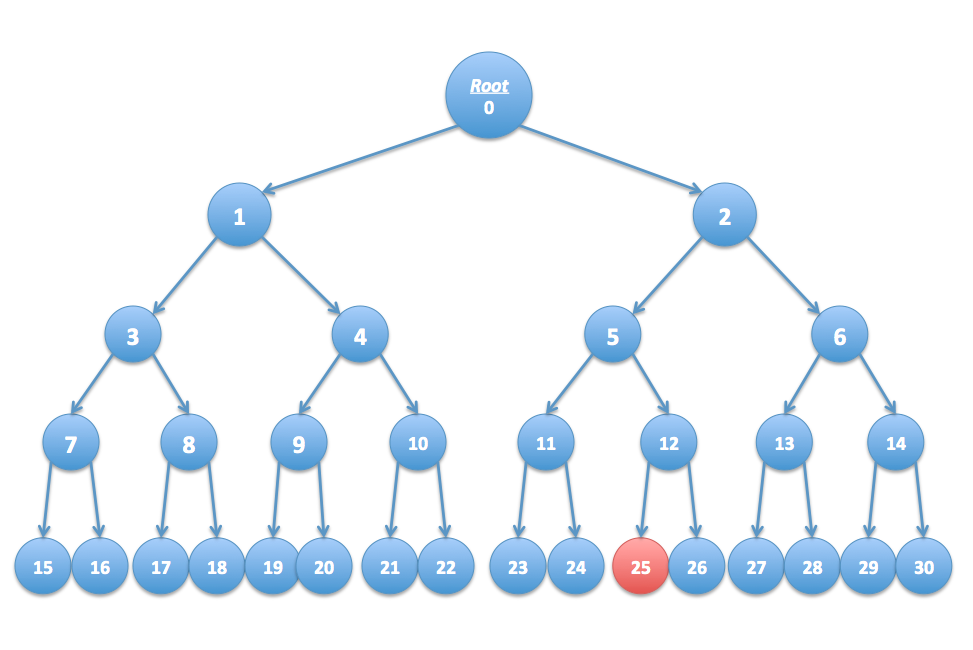
\includegraphics[scale=0.4]{question8-tree.png}
\end{center}

\textbf{Solution}\\

The keys are:
%
\begin{itemize}
\item $1$. You cannot encrypt $k$ under the root, but $1$'s children must be able to decrypt $k$.
\item $6$. You cannot encrypt $k$ under key $2$, but $6$'s children must be able to decrypt $k$.
\item $11$. You cannot encrypt $k$ under key $5$, but $11$'s children must be able to decrypt $k$.
\item $26$. You cannot encrypt $k$ under any key on the path from the root to node $25$. Therefore $26$ can only decrypt if you encrypt $k$ under key $k_{26}$.
\end{itemize}

%
\begin{itemize}
\item $4$. There is a better solution that does not require encrypting on the key of this node.
\item $15$. There is a better solution that does not require encrypting on the key of this node.
\item $18$. There is a better solution that does not require encrypting on the key of this node.
\item $19$. No, this will let node 25 decrypt the DVD.
\end{itemize}

\textbf{Question 9} \\

Continuing with the previous question, if there are n DVD players, what is the number of keys under which the content key k must be encrypted if exactly one DVD player's key needs to be revoked?
%
\begin{itemize}
%
\item $\frac{n}{2}$
\item $n - 1$
\item $2$
\item $\sqrt{n}$
\item $\log_{2}{n}$
%
\end{itemize}

\textbf{Solution} 

\begin{itemize}
%
\item $\log_{2}{n}$
%
\end{itemize}
%
That's right. The key will need to be encrypted under one key for each node on the path from the root to the revoked leaf. There are $\log_{2}{n}$ nodes on the path.

\textbf{Question 10}\\

Continuing with question 8, suppose the leaf nodes labeled $16$, $18$, and $25$ correspond to exposed DVD player keys. Check the smallest set of keys under which to encrypt the key $k$ so that every player other than players $16$, $18$ and $25$ can decrypt the DVD. Only six keys are needed.
%
\begin{enumerate}
\item $26$
\item $11$
\item $4$
\item $2$
\item $21$
\item $6$
\item $27$
\item $17$
\item $15$
\item $9$
\end{enumerate}

\textbf{Solution} \\

The smallest set of keys under which to encrypt the key $k$ so that every player other than players $16$, $18$ and $25$ can decrypt the DVD:
%
\begin{enumerate}
\item $4$. Yes, this will let players $19 - 22$ decrypt.
\item $6$. Yes, this will let players $27 - 30$ decrypt.
\item $11$. Yes, this will let players $23$ and $24$ decrypt.
\item $15$. Yes, this will let player $15$ decrypt.
\item $17$. Yes, this will let player $17$ decrypt.
\item $26$. Yes, this will let player $26$ decrypt.
\end{enumerate}
%
Those ones are not required:
%
\begin{enumerate}
\item $2$. No, this will let player $25$ decrypt.
\item $9$.
\item $21$.
\item $27$. 
\end{enumerate}

\end{document}
